\documentclass{beamer} 
\usepackage{amsmath,amsthm}
\usepackage{graphicx,microtype,parskip}
\usepackage{caption,subcaption,multirow}
\usepackage{attrib}

\frenchspacing

\usetheme{default}
\usecolortheme{whale}

\setbeamertemplate{navigation symbols}{}

\setbeamercolor{title}{fg=blue,bg=white}

\setbeamercolor{block title}{fg=white,bg=gray}
\setbeamercolor{block body}{fg=black,bg=lightgray}

\setbeamercolor{block title alerted}{fg=white,bg=darkgray}
\setbeamercolor{block body alerted}{fg=black,bg=lightgray}


\title{Metacommunities, assembly, \(\alpha\) and \(\gamma\)}

\begin{document}

\begin{frame}
  \maketitle
\end{frame}

\begin{frame}
  \frametitle{Species distribution across multiple localities}

  \begin{block}{Questions}
    \begin{itemize}
      \item How do mammal species traits effect co-occurrence patterns?
      \item What is the expected proportion of the mammal metacommunity pool present at a single locality?
      \item Have these relationships changed over the Cenozoic?
    \end{itemize}
  \end{block}
\end{frame}

\begin{frame}
  \frametitle{System}

  \begin{columns}
    \begin{column}{0.5\textwidth}
      \begin{itemize}
        \item Record
          \begin{itemize}
            \item North American Cenozoic
            \item 2 My bins
          \end{itemize}
        \item Units
          \begin{itemize}
            \item mammal species 
            \item 2x2 Lat-Long equal area grid cells
          \end{itemize}
        \item Covariates
          \begin{itemize}
            \item taxa: diet, locomotor, body size
            \item localities: ??
          \end{itemize}
        \item Hierarchical effects
          \begin{itemize}
            \item spatial relation
            \item phylogeny
          \end{itemize}
      \end{itemize}
    \end{column}
    \begin{column}{0.5\textwidth}
      \begin{itemize}
        \item Relations to community assembly
        \item Covariate hypotheses
          \begin{itemize}
            \item carnivore greatest diet co-occur
            \item ground dwelling \(>\) scansorial \(>\) arboreal
            \item body size: positive
          \end{itemize}
        \item Hierarchical effect interpretations
          \begin{itemize}
            \item spatial effect: \\structured vs random
            \item phylogeny: attract vs repel
          \end{itemize}
      \end{itemize}
    \end{column}
  \end{columns}
\end{frame}

\begin{frame}
  \frametitle{Bipartite network}
  \begin{center}
    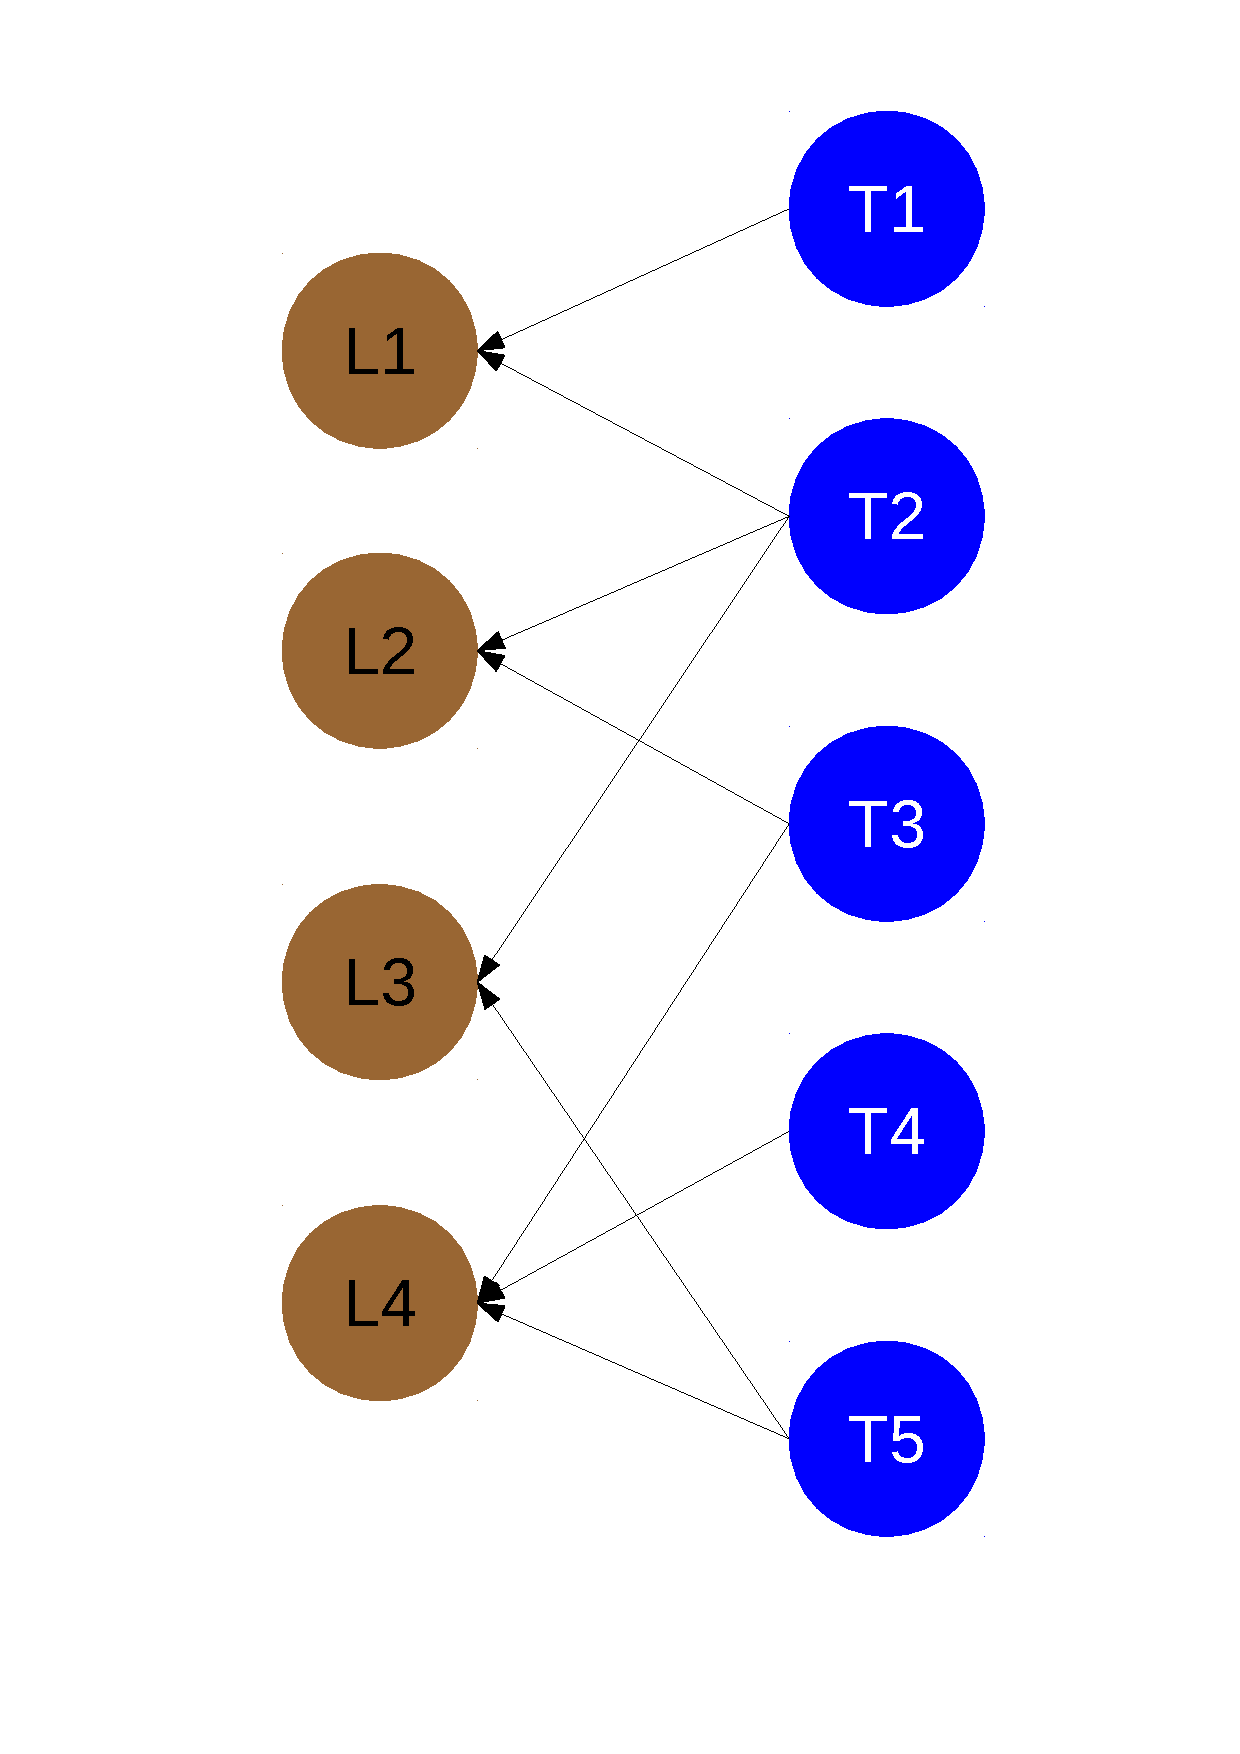
\includegraphics[height = 0.8\textheight, width = \textwidth,  keepaspectratio = true]{figure/bipartite_graph}
  \end{center}
\end{frame}

\begin{frame}
  \frametitle{One-mode network}
  \begin{center}
    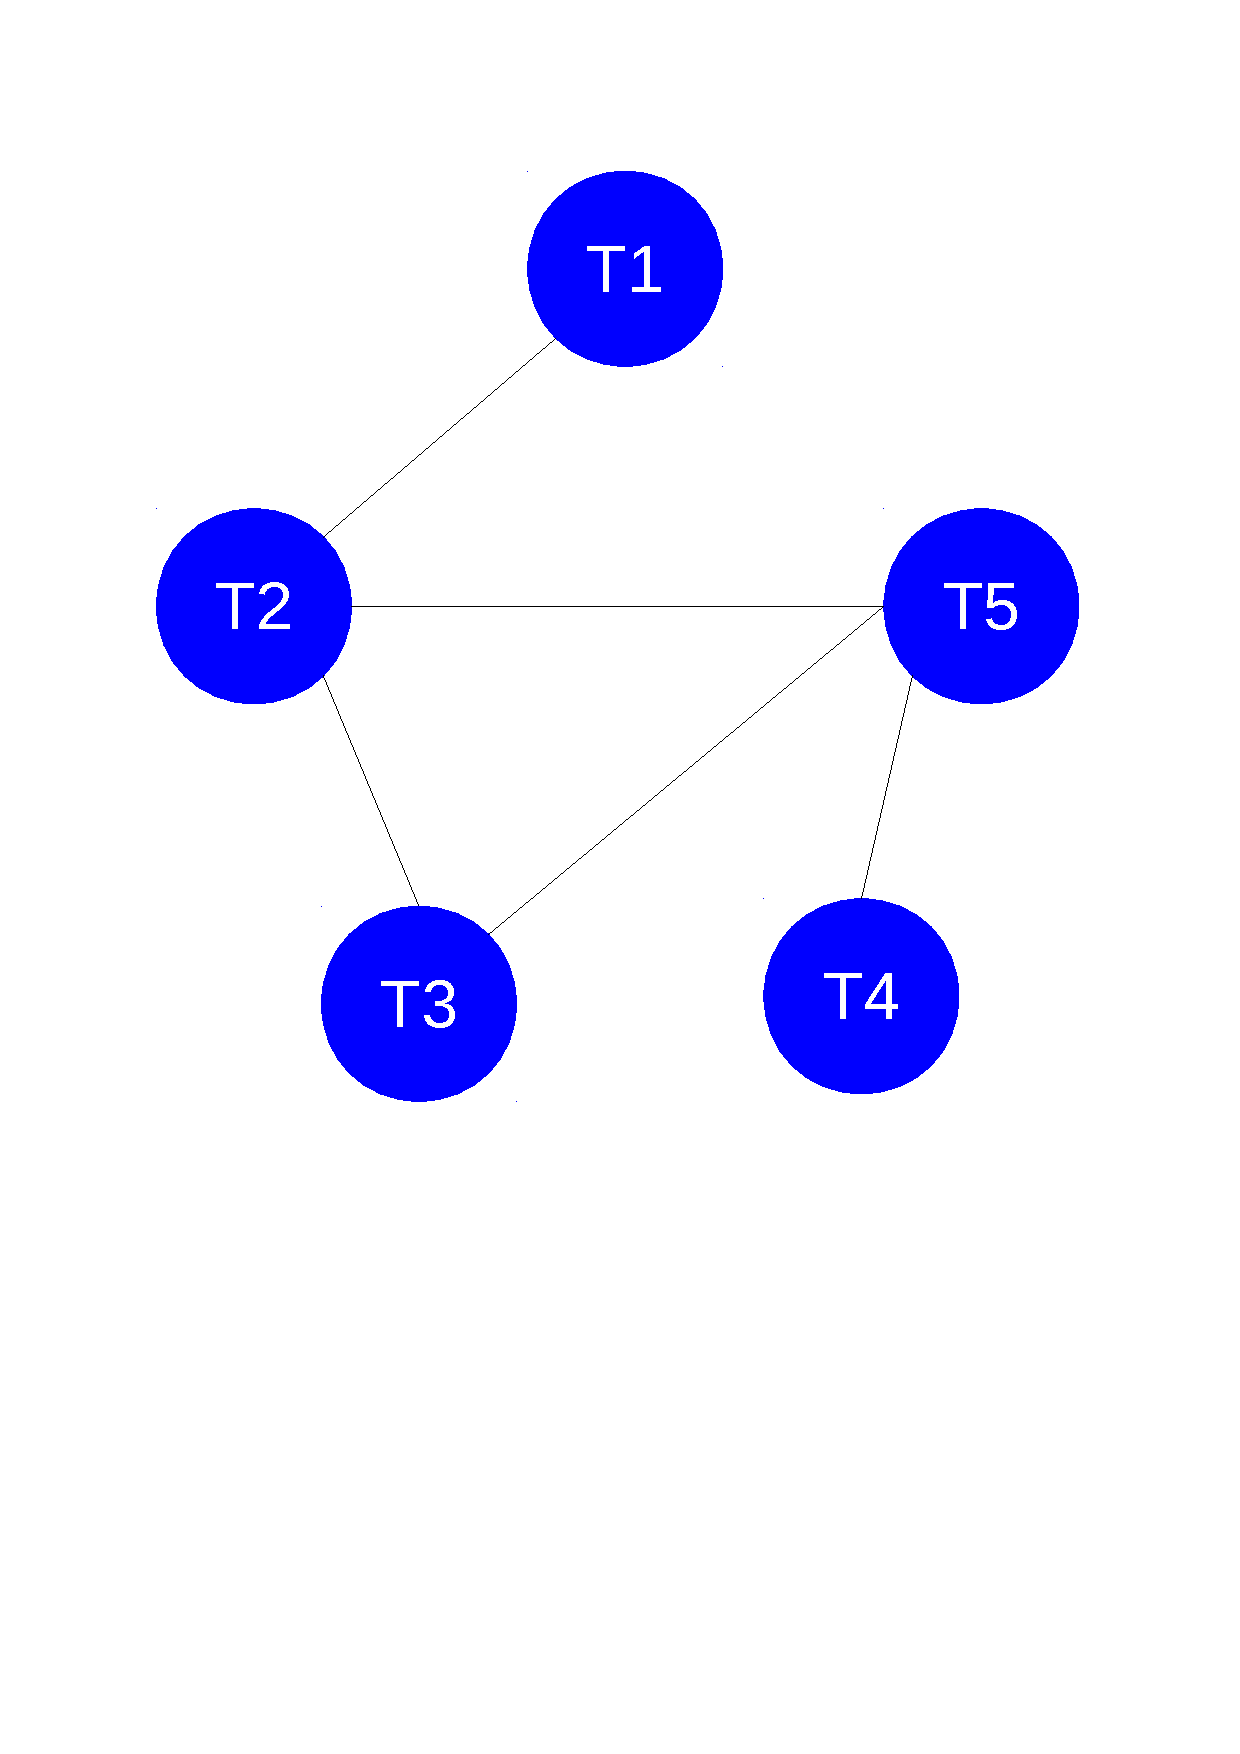
\includegraphics[height = 0.8\textheight, width = \textwidth,  keepaspectratio = true]{figure/one_mode}
  \end{center}
\end{frame}

\begin{frame}
  \frametitle{Modeling co-occurrence}
  \begin{alertblock}{Assumption and setup}
    \(y_{i}\): \# co-occurring species with species \(i\) per \# of localities.

    Any species is equally likely to co-occur with any other species.

    Consequence, node degree follows Poisson distribution \\(Erdos-Renyi random graph).
  \end{alertblock}
\end{frame}

\begin{frame}
  \frametitle{Modeling phylogenetic effect}
  \begin{definition}
    Assuming Brownian motion, effect drawn from multivariate normal distribution.

    \begin{equation*}
      h \sim \mathcal{N}(0, \sigma_{p}^{2}\mathbf{V_{p}})
    \end{equation*}

    \begin{itemize}
      \item Covariance known up to constant, \(\sigma_{p}\).
      \item \(\mathbf{V_{p}}\) phylogenetic covariance matrix (shared branch lengths).
    \end{itemize}

    \tiny{Follows Lynch 1991 \textit{Evolution}, Housworth \textit{et al.} 2004 \textit{Am. Nat.}}
  \end{definition}
\end{frame}

\begin{frame}
  \frametitle{Species co-occurrence model}
  \begin{center}
    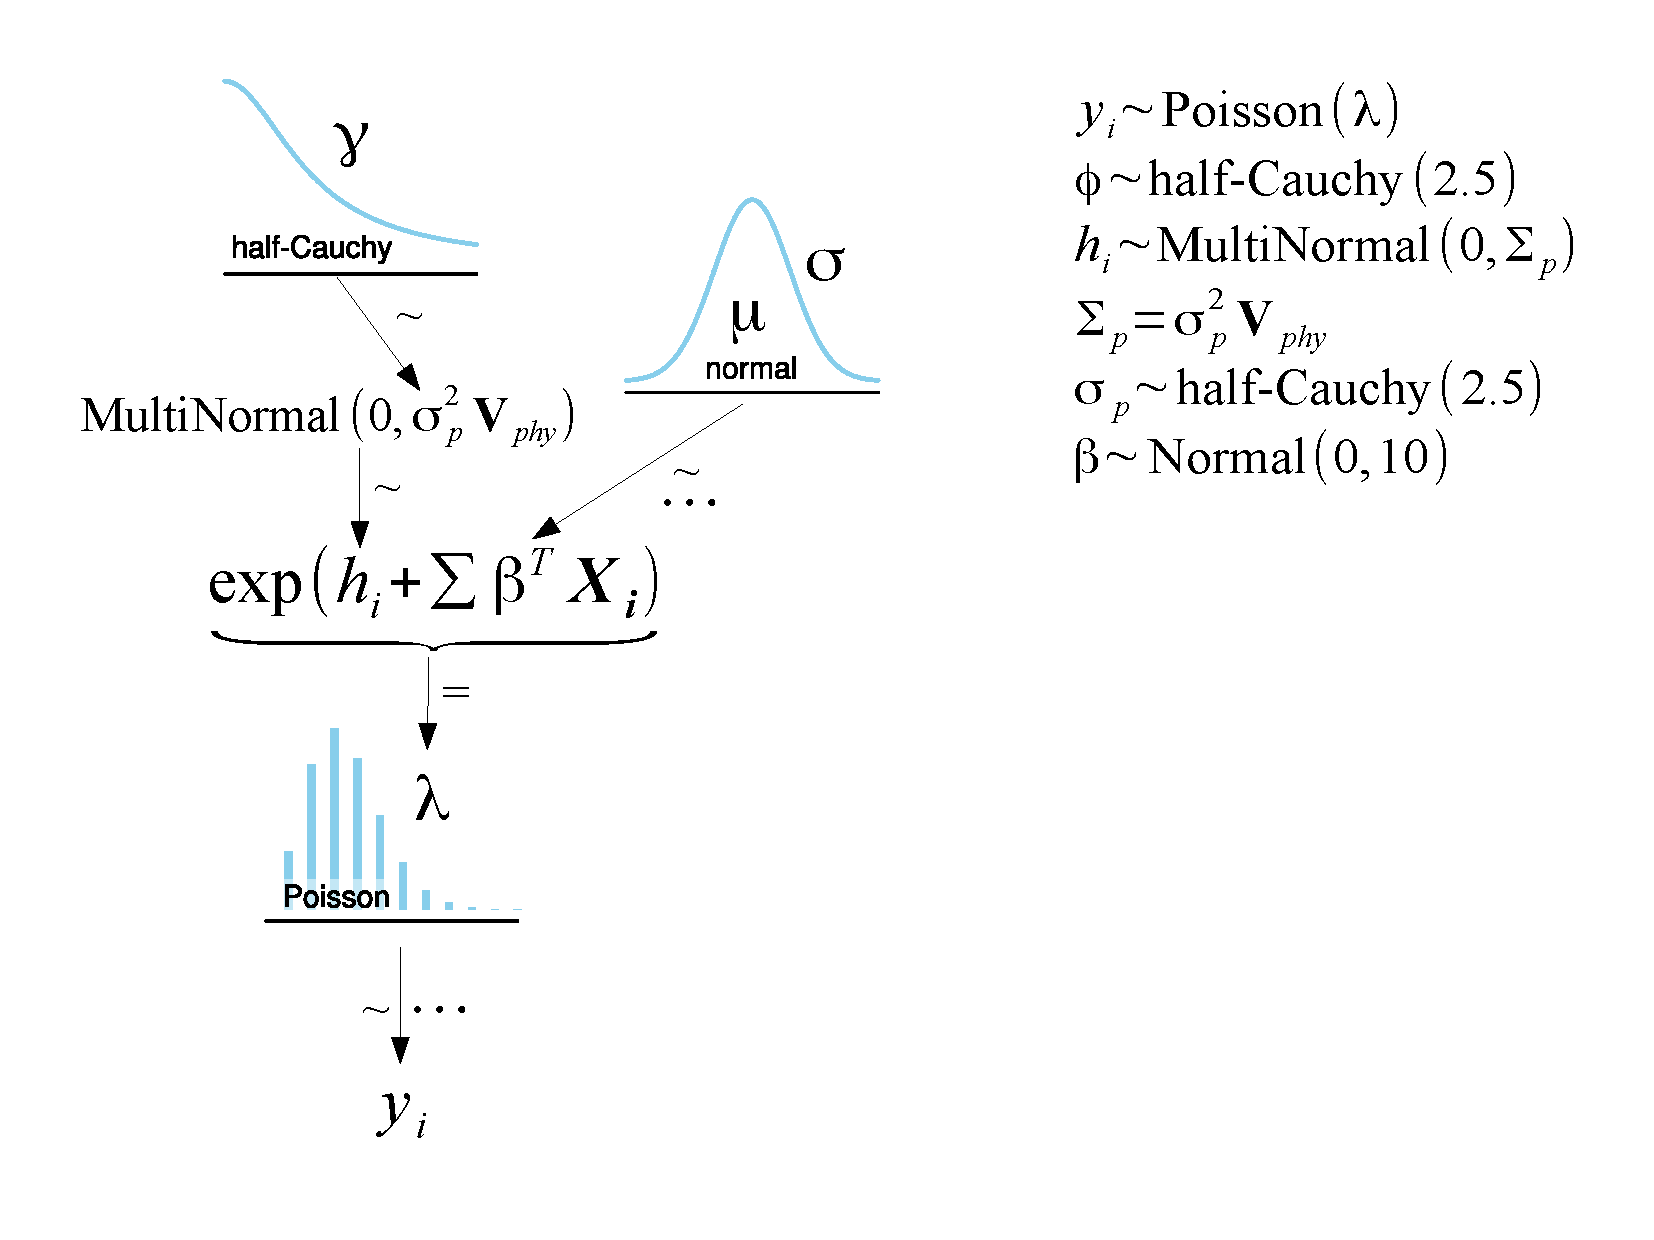
\includegraphics[height = 0.8\textheight, width = \textwidth,  keepaspectratio = true]{figure/mammal_degree_model}
  \end{center}
\end{frame}

\begin{frame}
  \frametitle{Modeling co-occurrence}
  \begin{block}{Improvement}
    Poisson assumption \(\frac{Var[x]}{E[x]} = 1\).

    Relax assumption by modeling overdisperssion \(\phi\).
  \end{block}
\end{frame}

\begin{frame}
  \frametitle{Species co-occurrence model redux}
  \begin{center}
    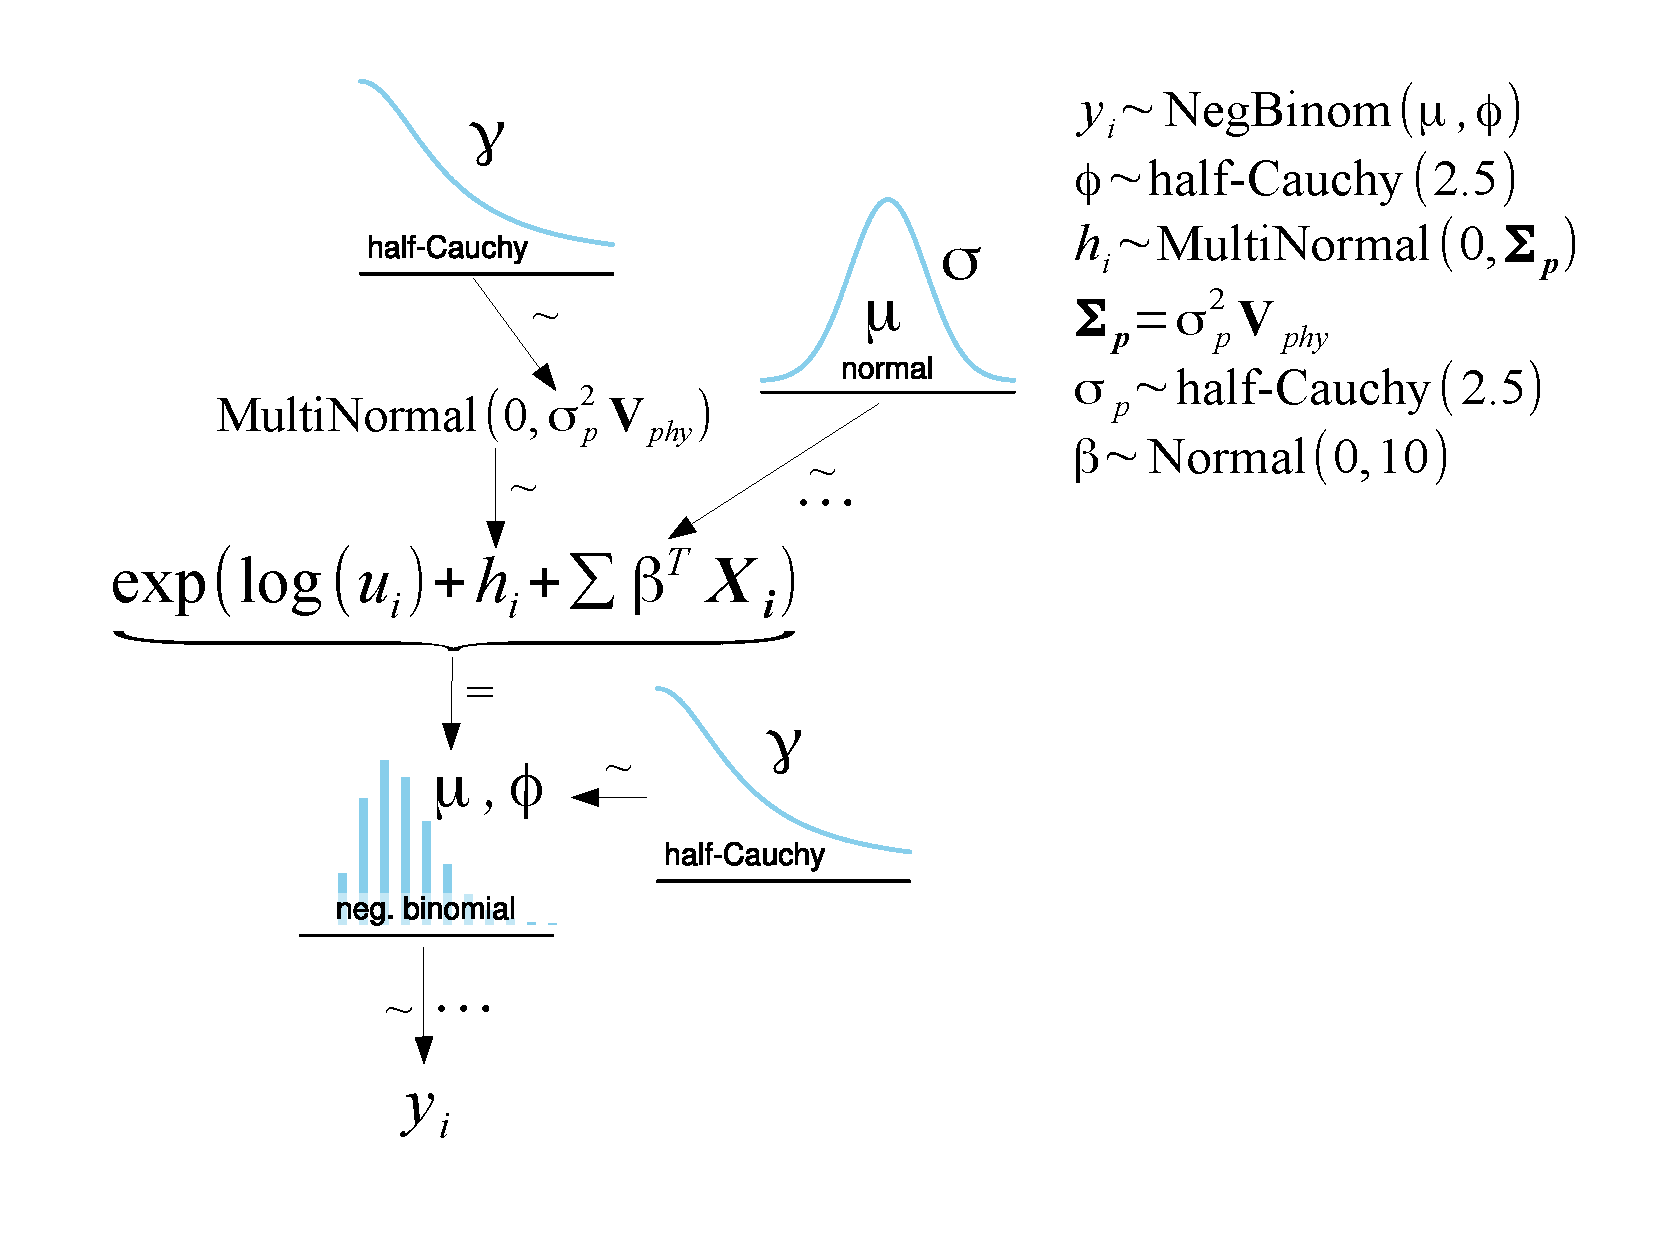
\includegraphics[height = 0.8\textheight, width = \textwidth,  keepaspectratio = true]{figure/mammal_deg_over_model}
  \end{center}
\end{frame}

\begin{frame}
  \frametitle{Modeling locality richness}
  \begin{alertblock}{Assumption and setup}
    \(y_{i}\): \# species at locality \(i\) per \# of species.

    \(y_{i}\) drawn from Poisson (or Negative Binomial) distribution.

    Localities are from non-uniform lattice (areal units).
  \end{alertblock}
\end{frame}

\begin{frame}
  \frametitle{Spatial effect}

  \begin{definition}
    Autoregressive prior; spatial effect drawn from multivariate normal.

    \begin{equation*}
      s \sim \mathcal{N}(0, \sigma_{s}^{2}(D - pA)^{-1})
    \end{equation*}

    \begin{itemize}
      \item \(\sigma_{s}\) is variance of spatial effect (size).
      \item \(D\) is diagonal matrix of neighbor count.
      \item \(A\) is adjacency matrix of localities.
      \item \(p\) is ``strength'' of spatial effect.
    \end{itemize}

    \tiny{Bunch of assorted problems regarding propriety. See Banerjee \textit{et al.} 2004 book.}

  \end{definition}
\end{frame}

\begin{frame}
  \frametitle{Locality richness model}
  \begin{center}
    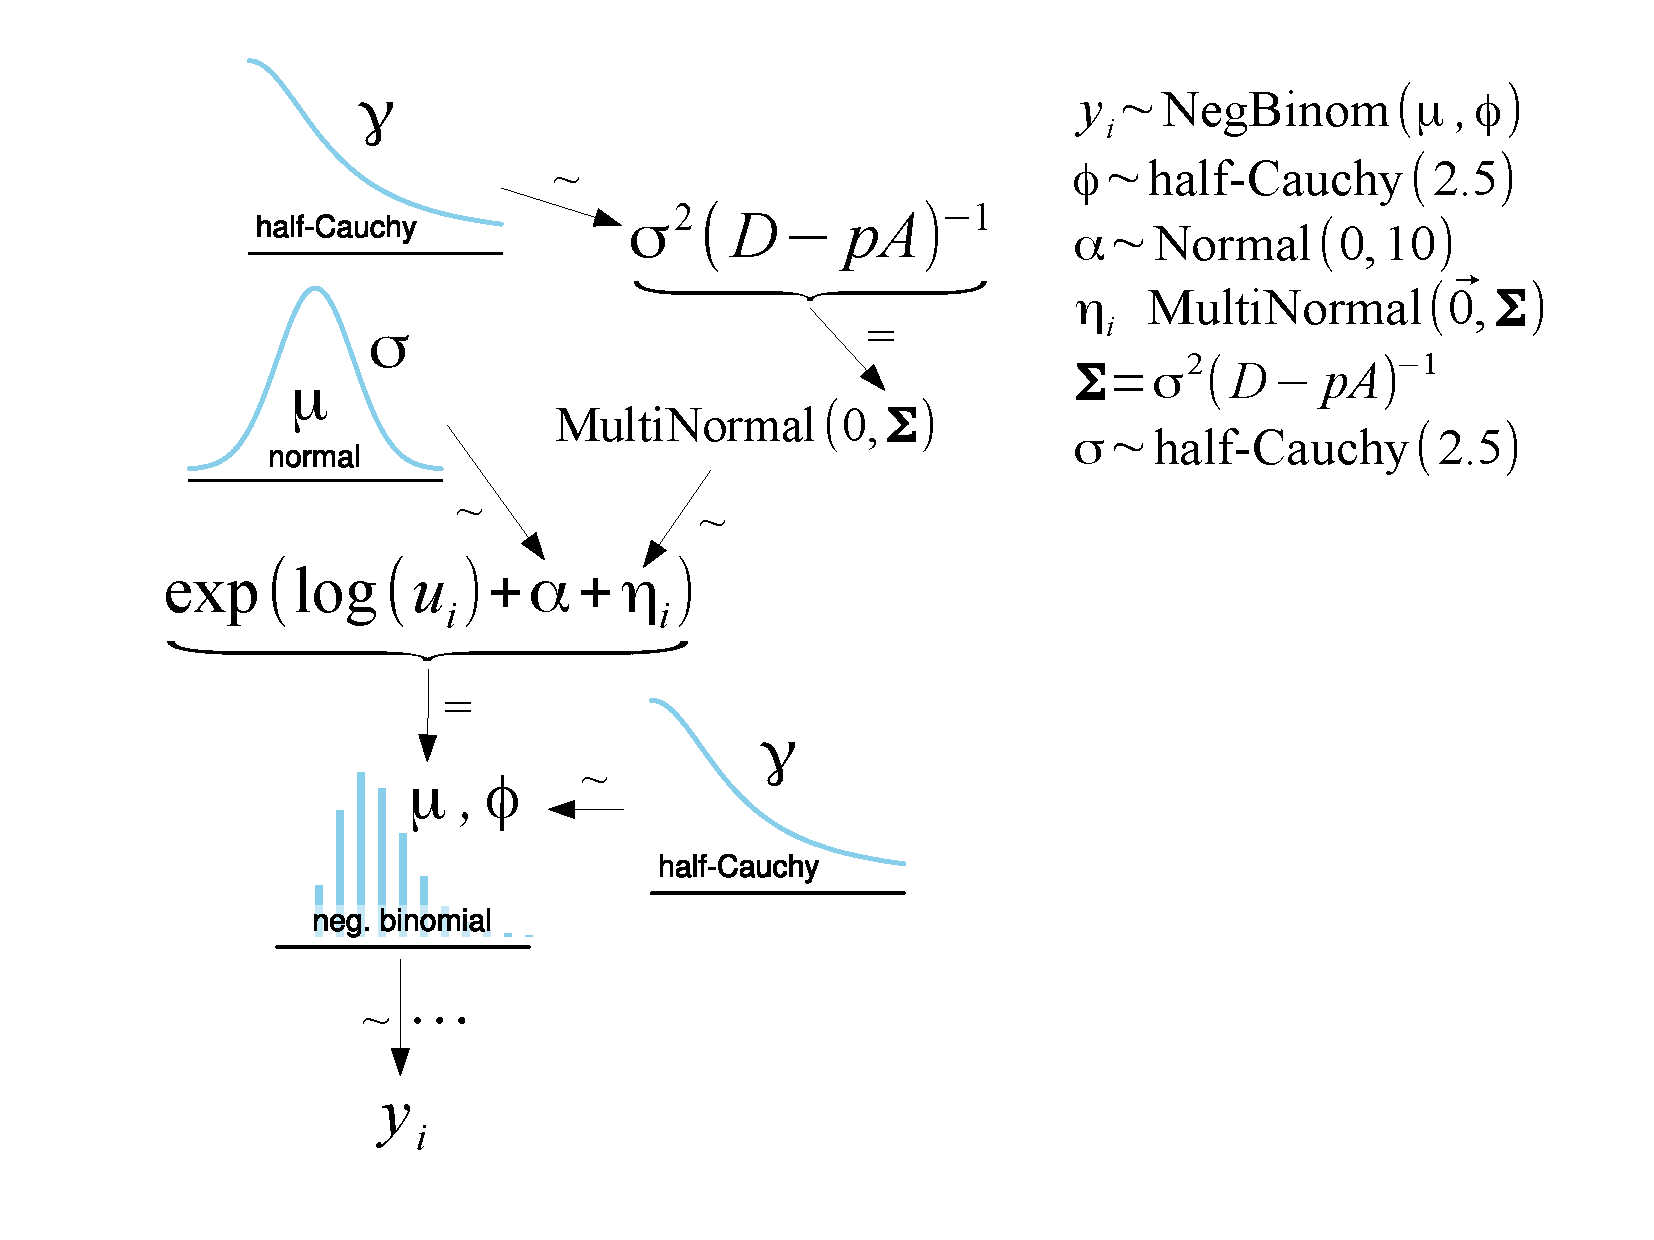
\includegraphics[height = 0.8\textheight, width = \textwidth,  keepaspectratio = true]{figure/mammal_locality_model}
  \end{center}
\end{frame}

\begin{frame}
  \frametitle{Analysis framework}
  \begin{center}
    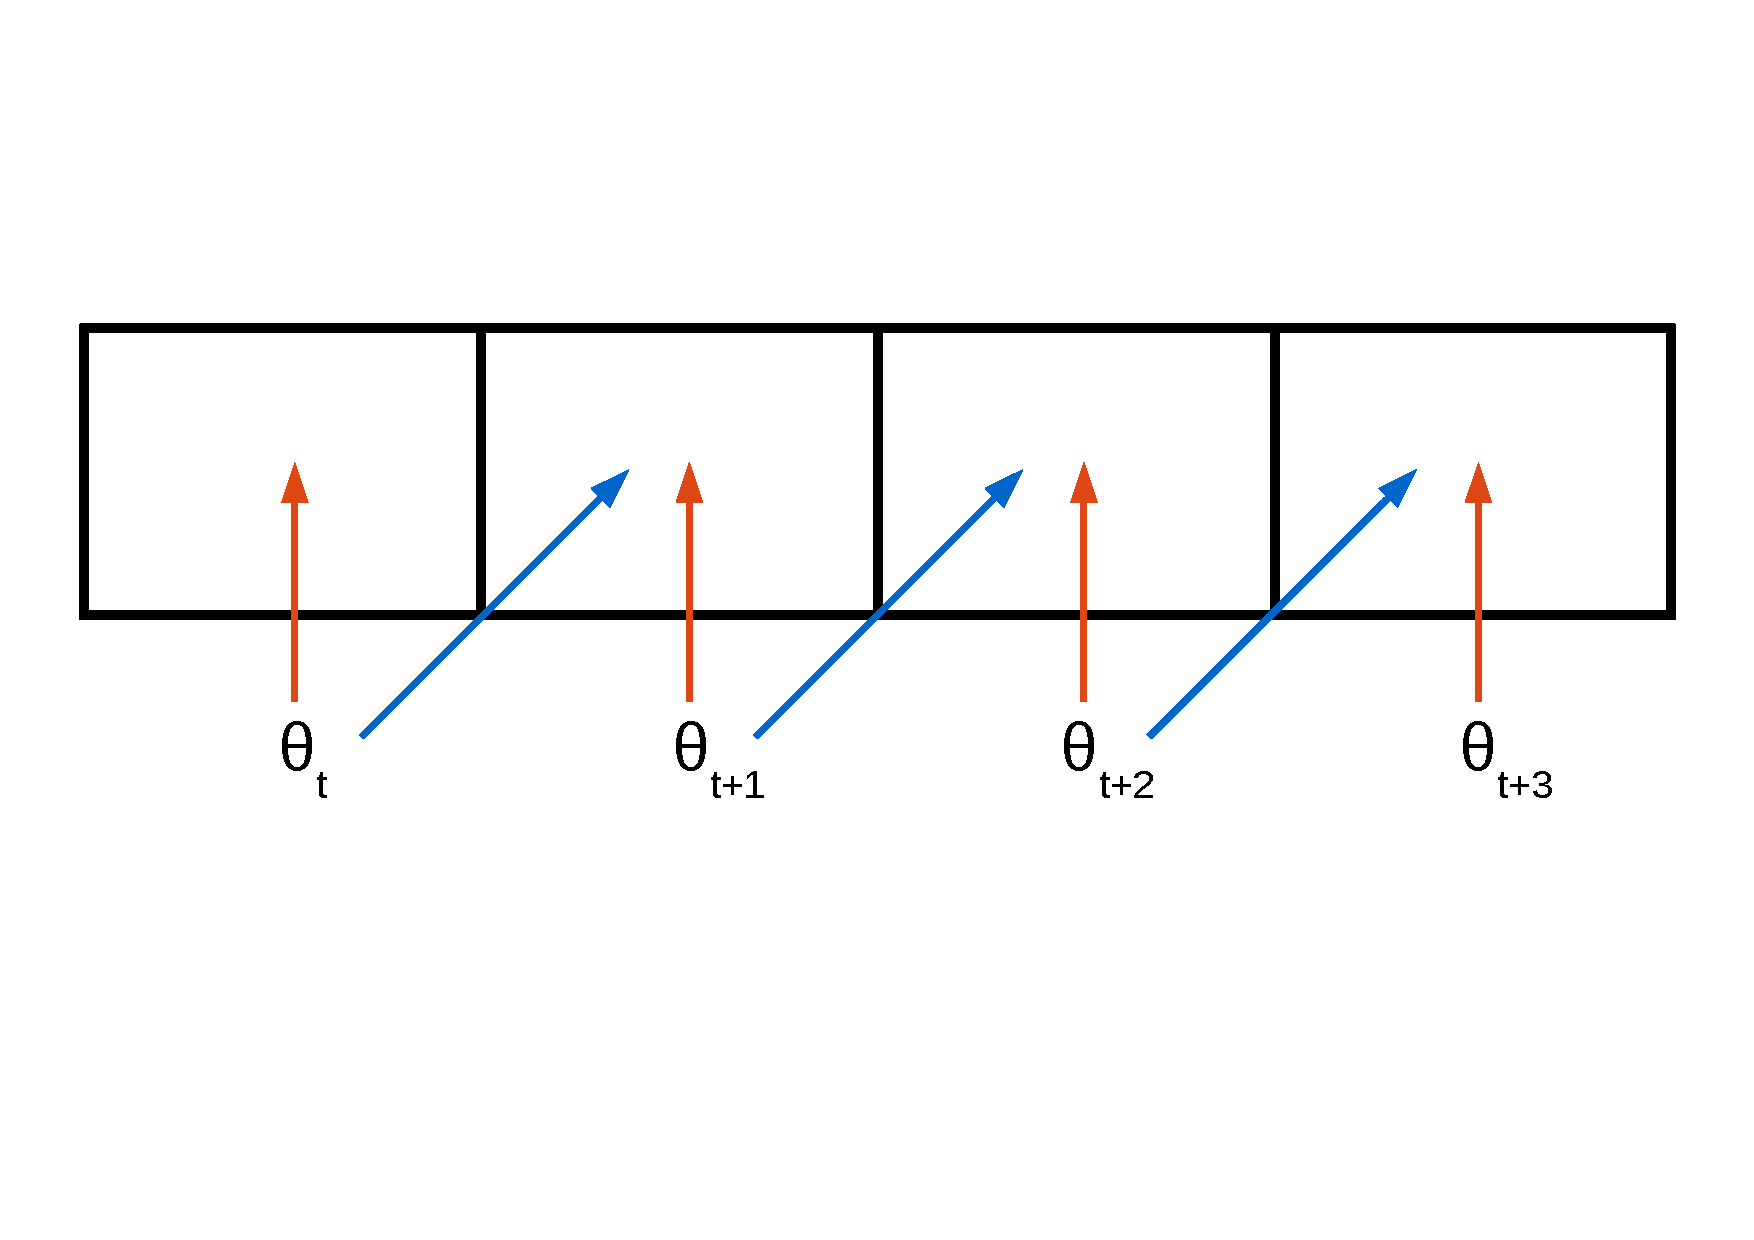
\includegraphics[height = 0.8\textheight, width = \textwidth,  keepaspectratio = true]{figure/predict_perform}
  \end{center}
\end{frame}

\end{document}
